\documentclass[12pt,a4paper]{article}
\usepackage[utf8]{inputenc}
\usepackage[italian]{babel}
\usepackage{amsthm}
\usepackage{amsmath}
\usepackage{mathtools}
\usepackage{booktabs}
\usepackage{tabularx}
\usepackage{multicol}
\usepackage{multirow}
\usepackage{graphicx}
\usepackage{fixltx2e}
\usepackage{mathrsfs}
\usepackage{amsfonts}
\usepackage{makeidx}
\usepackage[hidelinks]{hyperref}
\usepackage{relsize}
\usepackage{array}
\usepackage{fullpage}
\usepackage{dsfont}
\usepackage{amssymb}
\usepackage{attachfile}
\usepackage{eurosym}
\usepackage{tabto}
\usepackage{pifont}
\usepackage{tikz}
\usepackage{verbatim}
\usepackage{color,listings}
\usepackage{comment}
\usepackage{vwcol}  
\usepackage{lipsum}
\usepackage{microtype}
\usepackage{cleveref}
\usepackage{frcursive}
\usepackage[T1]{fontenc}
\usepackage{bbding}
\usepackage{pifont}
\newcommand\finline[3][]{\begin{myfont}[#1]{#2}#3\end{myfont}}%
\addto\captionsitalian{\renewcommand{\appendixname}{Allegato}}
\newcommand{\xmark}{\ding{55}}%

\usetikzlibrary{calc}
\usetikzlibrary{shapes,arrows}
\usetikzlibrary{automata,positioning}

\tikzstyle{block} = [draw, fill=blue!20, rectangle, 
    minimum height=3em, minimum width=6em, align=center]
\tikzstyle{dblock} = [block,double,double distance = 0.1em]
\tikzstyle{sblock} = [block,dashed]
\tikzstyle{sum} = [draw, fill=blue!20, circle, node distance=1cm]
\tikzstyle{pinstyle} = [pin edge={to-,thin,black}]
\tikzstyle{nlabel} = [above,pos=0.5,anchor=center,align=center]
\tikzstyle{nslabel} = [nlabel,sloped]
\tikzstyle{label} = [nlabel,fill=white,inner sep=1pt]
\tikzstyle{slabel} = [label,sloped]
\tikzstyle{arr} = [->, rounded corners]

\begin{document}

\begin{titlepage}
\begin{center}
\vspace{3cm}

\begin{center}

\includegraphics[scale=0.3]{Cherubino.jpg}
\end{center}

\vspace{1.5cm}

\Huge
{\sc Laboratorio di Sistemi Operativi}\\
\Large
Anno Accademico 2016/2017\\

\vspace{1cm}
\huge
{\sc Chatterbox}\\

\vspace{1.5cm}

\Large
A cura di\\
{\sc Gemma Martini}\\

\vspace{1.5cm}

\today

\vfill

\end{center}
\end{titlepage}

%%%%%%%%%%%%%%%%%%%~~~~~~~~~~~~~~~~~~~~~~~~~~~~~~~~~~~~~~~~~~~%%%%%%%%%%%%%%%%%%%%%

\tableofcontents
\newpage

%%%%%%%%%%%%%%%%%%%~~~~~~~~~~~~~~~~~~~~~~~~~~~~~~~~~~~~~~~~~~~%%%%%%%%%%%%%%%%%%%%%
							
\section{Introduzione}
Il software descritto in questo documento si occupa di gestire le funzionalità di un server per la gestione di una chat. Il comportamento ottenuto è quello di permettere ad un individuo di registrarsi, deregistrarsi, effettuare login e logout. Un volta iniziata la sessione l'utente può inviare messaggi testuali e file ad altri utenti e chiedere di vedere se gli è arrivato qualcosa mentre era offline. Una volta ricevuta tale lista, in caso di file, l'utente può richiederne lo scaricamento.
Per la realizzazione del programma sono state implementate un minimo di funzioni utilizzate dai client per l'impacchettamento dei messaggi.

%%%%%%%%%%%%%%%%%%%~~~~~~~~~~~~~~~~~~~~~~~~~~~~~~~~~~~~~~~~~~~%%%%%%%%%%%%%%%%%%%%%
							
\section{Scelte progettuali}
Durante lo sviluppo del codice si è proceduto iniziando la realizzazione delle parti che meno interagivano tra loro, così da permettere il testing quasi simultaneo alla scrittura, foriero di un numero inferiori di problemi in fase di testing finale.
Le scelte principali sono state le seguenti:
\begin{itemize}
\item In fase iniziale implementare delle liste generiche in modo da andare a rimorchio in tutta la stesura del codice;
\item Organizzare il codice un po' come un insieme di ``classi'', con i relativi ``metodi'' per rendere più chiara l'implementazione e la lettura da parte di terzi;
\item Effettuare la comunicazione dei task da eseguire tra thread principale e worker thread della thread pool mediante due code, una in una direzione ed una nell'altra;
\item Utilizzare delle ``select'' (sono in realtà state usate le \texttt{poll}, che non richiedono un numero massimo di elementi dell'array) per evitare al thread principale inutili attese (potenzialmente fatali);
\item Sostituire i signal handler con i \texttt{signalfd}, così da poter sfruttare al meglio le poll dando loro l'ulteriore compito di controllare la presenza di segnali pendenti, in sostituzione al normale meccanismo di gestione con chiamate asincrone;
\item Sostituire le condition variables con dei semafori (\texttt{eventfd}), così da poter sfruttare al meglio le poll dando loro l'ulteriore compito di controllare la presenza di almeno un elemento nella coda proveniente dalla thread pool.
\end{itemize}

\subsection{Più in dettaglio}
Durante la scrittura del codice sono state fatte delle scelte e delle assunzioni su parti specifiche del programma. In questa sezione vengono illustrate le decisioni prese:
\begin{itemize}
\item Durante l'invio di un messaggio di errore potrebbero verificarsi problemi, ad esempio la disconnessione del client. Nel file delle statistiche, il numero di messaggi di errore è il numero di messaggi di errore che sarebbero stati inviati, salvo errori imprevedibili;
\item Le statistiche contano il numero di messaggi inviati e da inviare e si è scelto di contare soltanto quelli testuali e non quelli che contengono file;
\item Ogni volta che si effettua una scrittura sul socket deve essere stato acquisito il lock su \texttt{server stuff}, così che non si mescolino risposte a varie richieste sullo stesso socket;
\item Gli errori delle funzioni di libreria e delle funzioni implementate ai fini del progetto sono stati gestiti solo quando si è ritenuto possibile il verificarsi di tali errori, infatti alcune funzioni falliscono sono in certi casi che, durante la stesura del codice sono stati evitati;
\item Per l'accesso alla struttura dati condivisa si è scelto di acquisire un lock prima di ogni operazione. Tale lock viene però rilasciato durante le operazioni di lettura e scrittura su disco;
\item Se un utente si disconnette senza fare logout la funzione \texttt{readAll} eseguita sul suo socket ritorna -1, così è possibile individuare l'evento e non rimanere bloccati a leggere. In tale eventualità, si è inoltre scelto di effettuare logout dell'utente. La disconnessione del client viene intercettata anche da \texttt{poll}.
\item Il ciclo di vita di un thread consta le seguenti parti:
	\begin{enumerate}
	\item Disattivazione dei segnali;
	\item Prelevamento di un socket da servire;
	\item Gestione di una singola richiesta;
	\item In caso non vi siano stati errori, inserimento del socket nella coda ``serviti'';
	\item Ripeti dal punto 2.
	\end{enumerate}
	Un thread della thread pool può essere cancellato soltanto durante la {\tt dequeue}, più precisamente durante la fase di attesa sul semaforo.
\end{itemize}

%%%%%%%%%%%%%%%%%%%~~~~~~~~~~~~~~~~~~~~~~~~~~~~~~~~~~~~~~~~~~~%%%%%%%%%%%%%%%%%%%%%
							
\section{Overview sul codice}
Il codice che, nella sua interezza, modella il funzionamento di \texttt{chatterbox} è stato realizzato seguendo uno stile di programmazione difensivo improntato alla suddivisione in ``classi'' concettuali (ossia in file muniti di strutture dati, funzioni e procedure). La figura \ref{fig:diagramma} fornisce un'idea grafica della struttura del software.
\begin{figure}
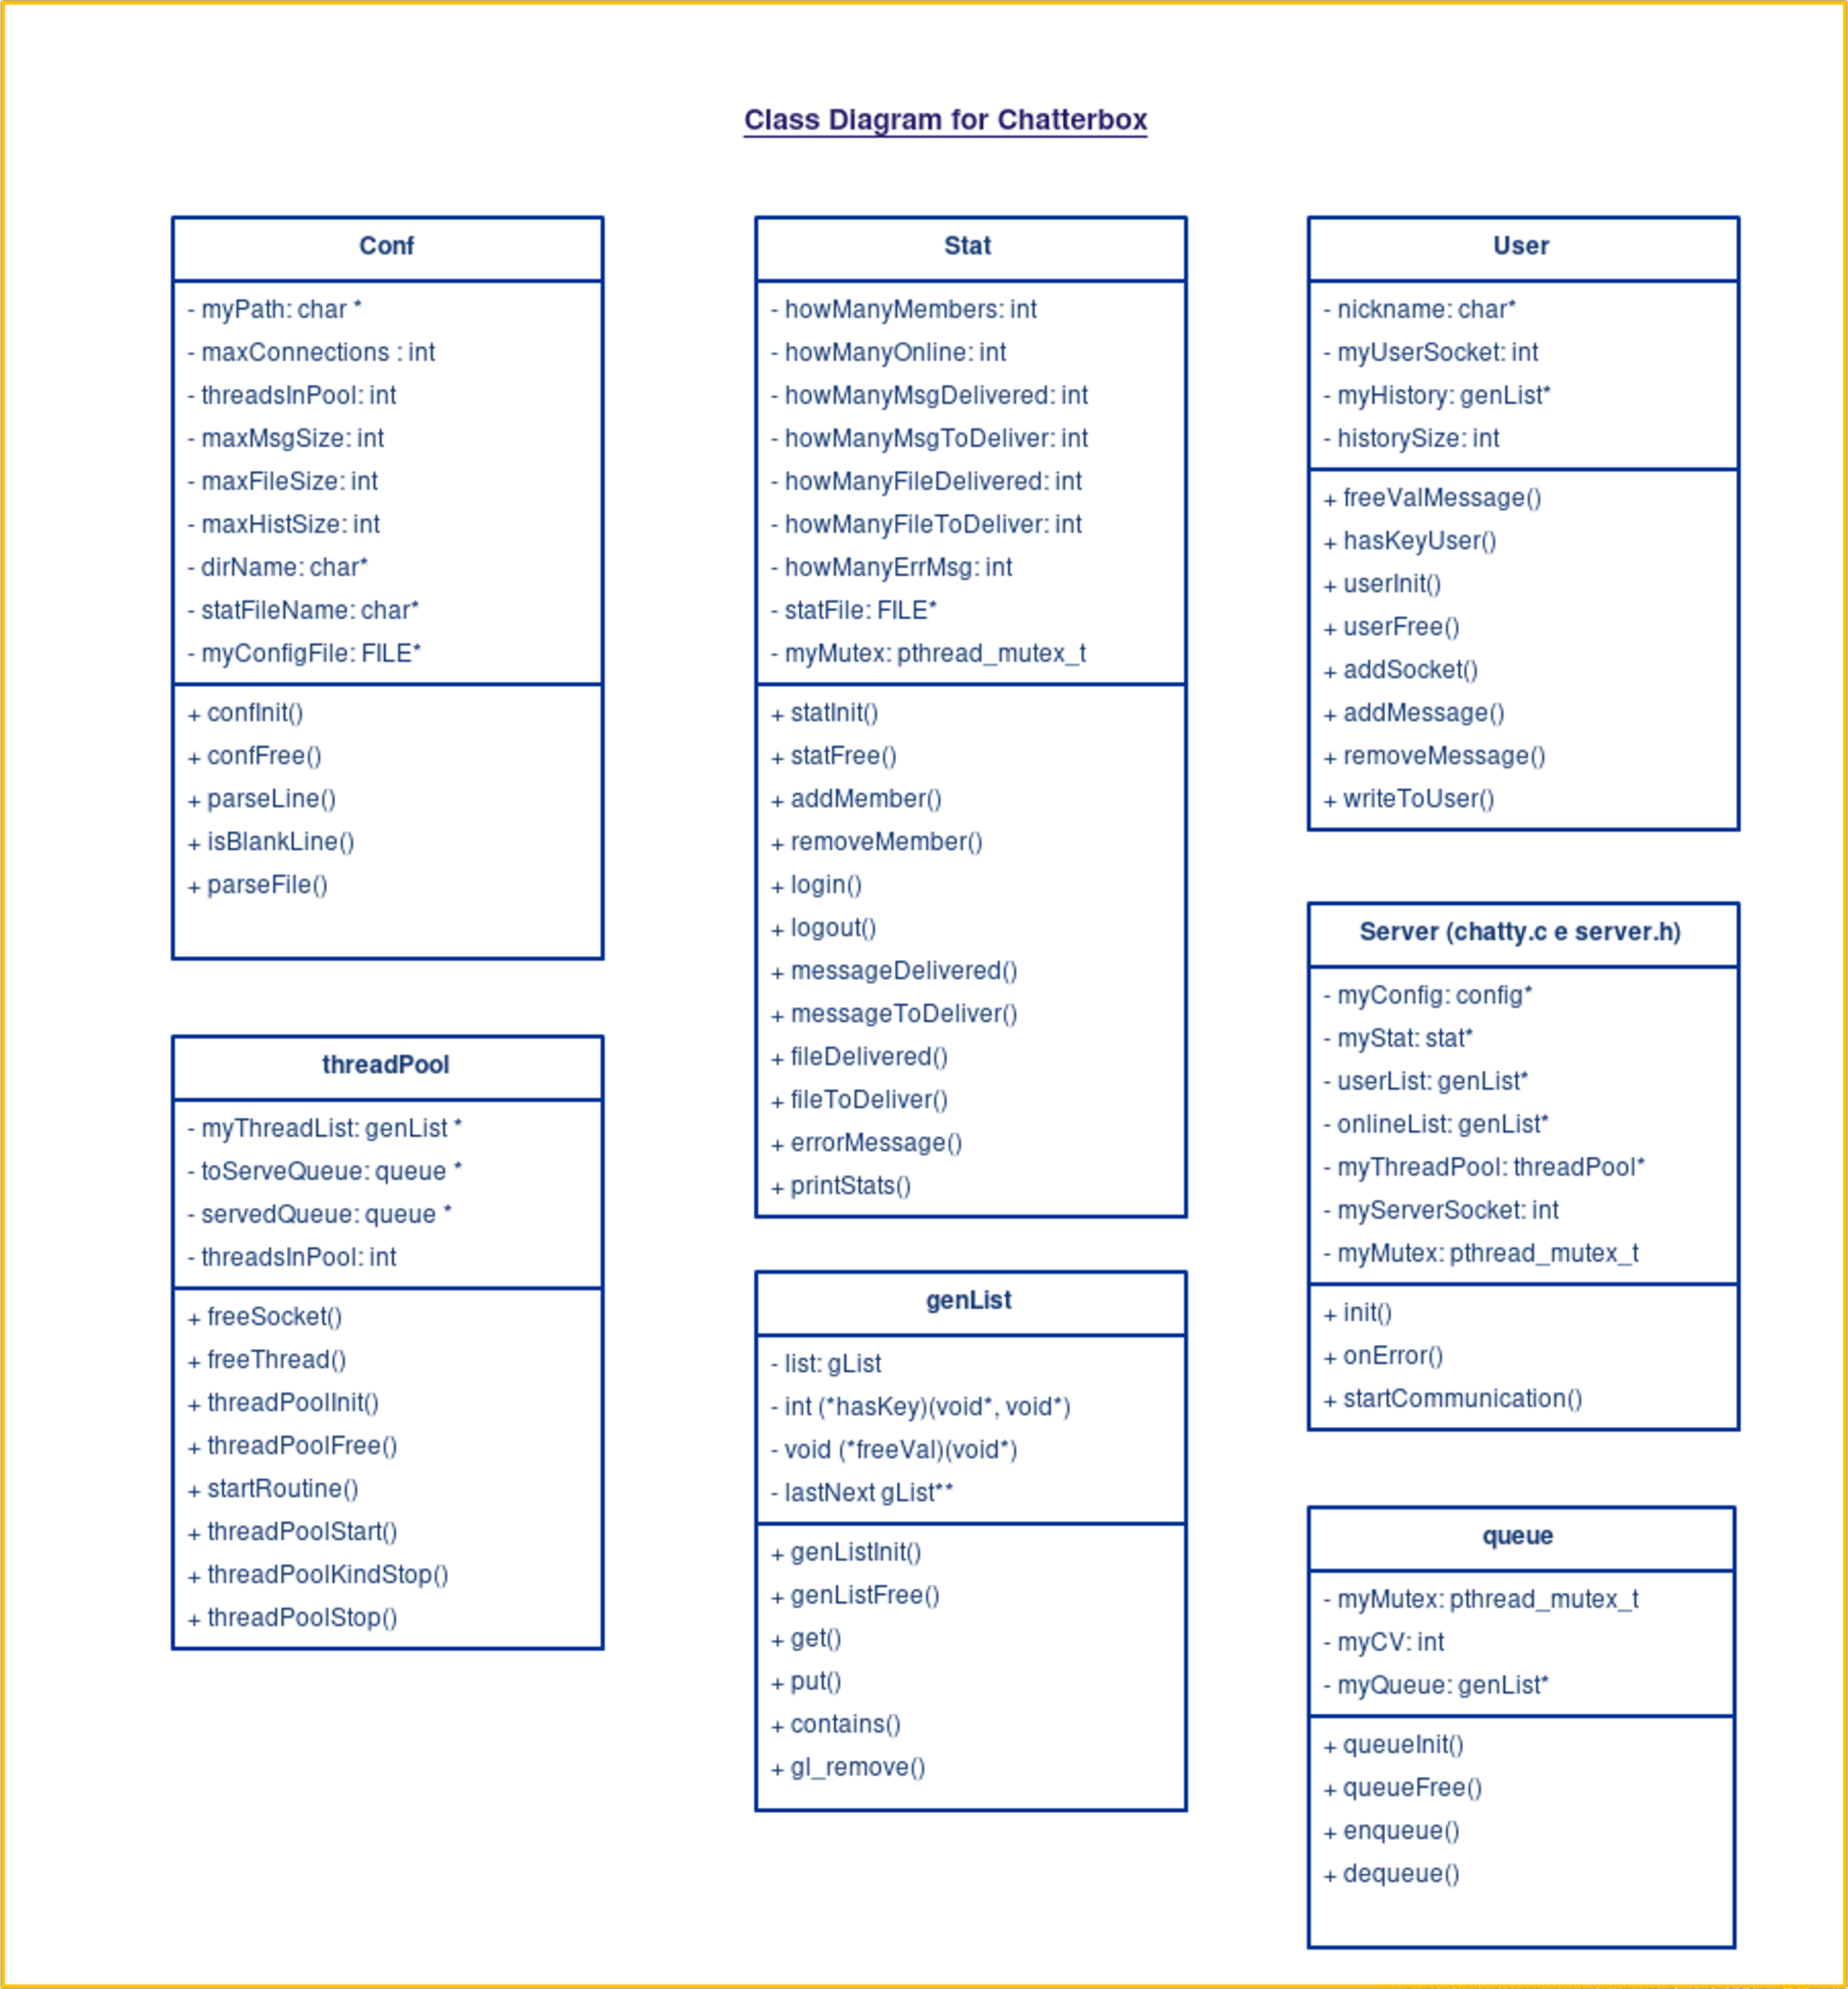
\includegraphics[width=\textwidth]{chatty.png}
\caption{Diagramma delle classi del progetto \label{fig:diagramma}}
\end{figure}
Oltre a tali classi vi è un file (\texttt{messageHandler.*}) che rappresenta un'interfaccia, ossia funzioni e procedure senza strutture dati collegate. 
Quel file implementa funzioni per la gestione delle varie operazioni richieste dai client, ma espone soltanto una funzione alla thread pool, ossia quella che, dato un messaggio, si occupa di passarlo al giusto handler.

%%%%%%%%%%%%%%%%%%%~~~~~~~~~~~~~~~~~~~~~~~~~~~~~~~~~~~~~~~~~~~%%%%%%%%%%%%%%%%%%%%%
							
\section{Difficoltà incontrate (e risolte)}
Durante lo sviluppo sono state incontrate alcune difficoltà:
\begin{itemize}
\item Comportamento inaspettato di {\tt client.c}: nella lettura dei messaggi di ``Operazione effettuata con successo'' ({\tt OP\_OK}) in alcune situazioni non veniva letto il body del messaggio. Tale comportamento lasciava dei dati nel socket, che inquinavano le letture successive. La soluzione è stata, quindi, modificare il funzionamento del client in modo da leggere sempre l'intero messaggio dal socket;
\item Comportamento inaspettato di {\tt client.c}, poichè in alcuni casi interpretava il ritorno di alcune funzioni (di quelle da implementare) come -1 in caso di errore, altrimenti successo, mentre in altri casi un numero positivo in caso di successo, un numero <= 0 in caso di errore. La soluzione è stata cambiare il funzionamento di tali funzioni da me implementate. In particolare, in caso di successo ritornano 1, che va bene in entrambi i casi;
\item Inizialmente si è scelto di comunicare la lista degli utenti online con l'operazione {\tt USRLIST\_OP}, ma il client voleva {\tt OK\_OP}, quindi si è cambiato in corso d'opera;
\item Inizialmente si pensava che l'invio di file avvenisse inviando un messaggio che conteneva il solo contenuto del file, lasciando al server la scelta del nome univoco di esso all'interno della cartella. Successivamente, in fase di testing, è stata riscontrata una differenza nel comportamento e si è provveduto alla modifica.
\end{itemize}

%%%%%%%%%%%%%%%%%%%~~~~~~~~~~~~~~~~~~~~~~~~~~~~~~~~~~~~~~~~~~~%%%%%%%%%%%%%%%%%%%%%
							
\section{Conclusioni}
Si conclude che il server progettato si confà alle richieste della committenza ed ai requisiti del progetto. La gestione della memoria avviene mediante l'uso puntuale di funzioni di cleanup associate alle varie strutture dati. La dipendenza delle varie funzioni l'una dall'altra, così come ulteriori dettagli di implementazione, sono facilmente reperibili del file doxygen qui allegato \attachfile{../doc/latex/refman.pdf}.

\end{document}
    
